\documentclass{standalone}
\usepackage{tikz-network}
\begin{document}
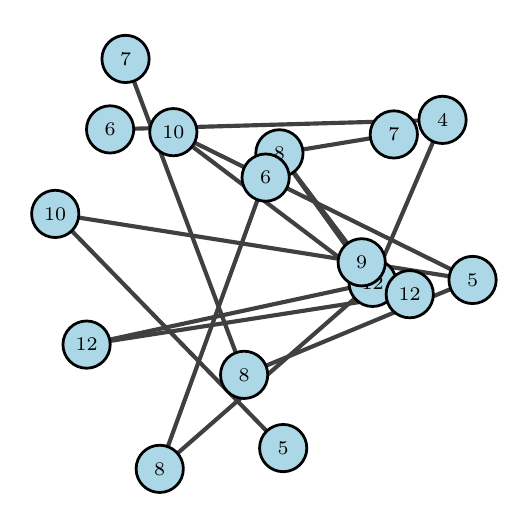
\begin{tikzpicture}
\clip (0,0) rectangle (6,6);
\Vertex[x=1.850,y=4.673,label=10]{1}
\Vertex[x=4.381,y=2.759,label=12]{7}
\Vertex[x=5.650,y=2.796,label=5]{2}
\Vertex[x=3.197,y=4.404,label=8]{8}
\Vertex[x=5.269,y=4.829,label=4]{11}
\Vertex[x=0.748,y=1.975,label=12]{15}
\Vertex[x=4.852,y=2.615,label=12]{16}
\Vertex[x=2.749,y=1.591,label=8]{3}
\Vertex[x=1.243,y=5.603,label=7]{4}
\Vertex[x=0.350,y=3.635,label=10]{5}
\Vertex[x=3.245,y=0.661,label=5]{6}
\Vertex[x=1.677,y=0.397,label=8]{13}
\Vertex[x=3.022,y=4.096,label=6]{14}
\Vertex[x=1.047,y=4.708,label=6]{12}
\Vertex[x=4.650,y=4.644,label=7]{10}
\Vertex[x=4.242,y=3.020,label=9]{9}
\Edge[](1)(7)
\Edge[](1)(2)
\Edge[](7)(8)
\Edge[](7)(11)
\Edge[](7)(15)
\Edge[](7)(13)
\Edge[](2)(5)
\Edge[](2)(3)
\Edge[](8)(10)
\Edge[](8)(9)
\Edge[](11)(12)
\Edge[](15)(16)
\Edge[](3)(4)
\Edge[](5)(6)
\Edge[](13)(14)
\end{tikzpicture}
\end{document}